% ------------------------------------------------------------------------------
% OpenQuake Engine Book 
% 
% Authors: 
% 	H. Crowley 		- Executive Committee - GEM Foundation, Pavia, Italy
% 	D. Monelli 		- GEM Model Facility, ETH-SED, Zurich, Switzerland
% 	M. Pagani 		- Executive Committee - GEM Foundation, Pavia, Italy
% 	V. Silva 		- GEM Model Facility, Pavia, Italy
%	G. Weatherhill 	- GEM Model Facility, Pavia, Italy
% 
% Document distributed under the Common Creative License 
% © GEM Foundation, Pavia, February 2011
% ------------------------------------------------------------------------------
\documentclass[11pt,a4paper,headings=small,dvips]{scrbook}
% --------------------------------------------------------------------- Packages
%%%%%%%%%%%%%%%%%%%%%%%%%%%%%%%%%%%%%%%%%%%%%%%%%%%%%%%%%%%%%%%%%%%%%%%%%%%%%%%%
% The GEM Technical Documentation LaTeX Template
% Version 1.0 (12/4/14)
%
% Original author:
% Mathias Legrand (legrand.mathias@gmail.com)
%
% Adapted for use by the GEM Foundation by:
% James Brown (james.brown@globalquakemodel.org)
% Anirudh Rao (anirudh.rao@globalquakemodel.org)
%
% License:
% CC BY-NC-SA 3.0 (http://creativecommons.org/licenses/by-nc-sa/3.0/)
%
% Compiling this template:
% This template uses bibtex for its bibliography and makeindex for its index.
% When you first open the template, compile it from the command line with the
% commands below to make sure your LaTeX distribution is configured correctly:
%
% 1) pdflatex -interaction=nonstopmode oq-manual.tex
% 2) bibtex oq-manual
% 3) pdflatex -interaction=nonstopmode oq-manual.tex
% 4) pdflatex -interaction=nonstopmode oq-manual.tex
% 5) makeindex oq-manual.idx -s configuration/StyleInd.ist
% 6) makeglossaries oq-manual
% 7) pdflatex -interaction=nonstopmode oq-manual.tex
%
% After this, when you wish to update the bibliography/index use the appropriate
% command above and make sure to compile with pdflatex several times
% afterwards to propagate your changes to the document.
%
% This template also uses a number of packages which may need to be
% updated to the newest versions for the template to compile. It is strongly
% recommended you update your LaTeX distribution if you have any
% compilation errors.
%
% Important note:
% Chapter heading images should have a 2:1 width:height ratio,
% e.g. 920px width and 460px height.
%
%%%%%%%%%%%%%%%%%%%%%%%%%%%%%%%%%%%%%%%%%%%%%%%%%%%%%%%%%%%%%%%%%%%%%%%%%%%%%%%%

% Page layout and margins
\usepackage[top=3cm,bottom=3cm,left=3.2cm,right=3.2cm,headsep=10pt,a4paper]{geometry}
\linespread{1.25}

% Font settings
\usepackage[condensed]{roboto} % Use the Roboto font for headings
\usepackage[bitstream-charter]{mathdesign} % Use the Bitstream Charter font for text
% \usepackage{amsmath,amsfonts,amssymb,amsthm} % For math equations, theorems, symbols, etc
\usepackage{microtype} % Slightly tweak font spacing for aesthetics
\usepackage[utf8]{inputenc} % Required for including letters with accents
\usepackage[T1]{fontenc} % Use 8-bit encoding that has 256 glyphs

% Color settings
\usepackage{color, colortbl}
\usepackage{xcolor} % Required for specifying colors by name
\definecolor{oqblue}{RGB}{27,117,165} % From the GEM Brand Guidelines
\definecolor{darkblue}{rgb}{.2,.2,.8}
\definecolor{darkgray}{gray}{0.25}

% Bibliography settings
\usepackage{csquotes}
\usepackage[style=alphabetic,
            sorting=nyt,
            sortcites=true,
            natbib=true,
            style=authoryear,
            maxcitenames=2,
            maxbibnames=100,
            autopunct=true,
            autolang=hyphen,
            hyperref=true,
            doi=true,
            abbreviate=false,
            backref=true,
            backend=bibtex,
            bibencoding=ascii,
            firstinits=true,
	    	uniquename=false,
	    	uniquelist=false]{biblatex}
\addbibresource{bibliography/hazard.bib} % Hazard BibTeX bibliography file
\addbibresource{bibliography/risk.bib} % Risk BibTeX bibliography file
\defbibheading{bibempty}{}

% Figure caption settings
\usepackage[textfont=it,margin=10pt,font=small,labelfont=bf,labelsep=endash]{caption}
\usepackage{subcaption}

% Rotate any object
\usepackage{rotating}

% Verbatim environments
\usepackage{verbatim}
\usepackage{fancyvrb}

% Index settings
\usepackage{calc} % Infix notation for \setcounter, \addtocounter, \setlength, \addtolength
\usepackage{makeidx} % Required to make an index
\setcounter{secnumdepth}{3}
\setcounter{tocdepth}{3} % Entries down to \subsubsections in the TOC
\makeindex % Tells LaTeX to create the files required for indexing

\usepackage{todonotes}
\usepackage{marginnote}

% Access bold symbols in maths mode
\usepackage{bm}

% Flexible typesetting of tables and figures
\usepackage{ctable}
\usepackage{booktabs}

% Customization of section titles and table of contents
\usepackage{titlesec}
\usepackage{titletoc}

% Header and footer customization
\usepackage{fancyhdr}
\usepackage{etoolbox}

\usepackage{graphicx} % Required for including pictures
\usepackage{tikz} % Required for drawing custom shapes
\usepackage{eso-pic} % Required for specifying an image background in the title page
\usepackage{pdfpages} % Needed to load .pdf pages, used for the cover page

% English language hyphenation
\usepackage[english]{babel}

\usepackage{enumitem} % Customize lists
\setlist{nolistsep} % Reduce spacing between bullet points and numbered lists
\usepackage{listings} % Required for embedding code snippets

\usepackage{hyperref}
\hypersetup{hidelinks,colorlinks=true,breaklinks=true,citecolor=darkblue,linkcolor=darkgray,urlcolor=oqblue,bookmarksopen=false,pdftitle={Title},pdfauthor={Author}}

% Package to create a glossary - must be loaded after hyperref
\usepackage[acronym,nonumberlist,style=altlist]{glossaries}
\glstoctrue
\makeglossaries



%
% ------------------------------------------------------------------------------
\uppertitleback{
   \textbf{Authors:} \\
   Helen Crowley$^1$, Vitor Silva$^2$ \\ \hfill \\
   \small
   \begin{tabular}{p{4cm}p{4cm}p{4cm}}
   $^1$ GEM Foundation \hfill \newline
   via Ferrata, 1 \hfill \newline 
   20133 Pavia \hfill \newline
   Italy \hfill \newline
   & 
   $^2$ GEM Model Facility \hfill \newline 
   via Ferrata, 1 \hfill \newline 
   20133 Pavia \hfill \newline
   Italy \hfill \newline   
	\end{tabular} \hfill \newline
   %
	Email address (for all the authors):\hfill\\
   $<$name.surname$>$@globalquakemodel.org
   %
   \vspace{0.2cm} \hfill \\
   {\bf{Disclaimer}} \hfill \\
   The OpenQuake Engine Book is distributed in the hope that it will be useful, 
   but without any warranty: without even the implied warranty of 
   merchantability or fitness for a particular purpose. While every 
   precaution has been taken in the preparation of this document, in 
   no event shall the authors of the book and the GEM Foundation be 
   liable to any party for direct, indirect, special, incidental, or 
   consequential damages, including lost profits, arising out of the 
   use of information contained in this document or from the use of 
   programs and source code that may accompany it, even if the authors 
   and GEM Foundation have been advised of the possibility of such damage. 
   The Book provided hereunder is on as "as is" basis, and the authors 
   and GEM Foundation have no obligations to provide maintenance, support,
   updates, enhancements, or modifications. 
   \hfill \\
   The current version of the book has been revised only by members of 
   the GEM Model Facility and it must be considered a draft copy.
   %
   \vspace{0.2cm} \hfill \\
   {\bf{License}} \hfill \\
   This Book is distributed under the Creative Common License 
   Attribution 3.0 Unported (CC BY 3.0) 
   (see link below). You can download this Book and share it with others 
   as long as you provide proper 
   credit, but you cannot change it in any way.
   \hfill \\
   \href{http://creativecommons.org/licenses/by/3.0/}
   {http://creativecommons.org/licenses/by/3.0/}  
   
   \hfill \\
   {\bf{Credit}} \hfill \\
   Crowley, H., V. Silva (2013). OpenQuake Engine Book: Risk. GEM Foundation, Pavia, Italy.   
   \normalsize
}  
%
% =============================================================== BEGIN DOCUMENT
% -------------------------------------------------- Title and table of contents
\begin{document}
% - - - - - - - - - - - - - - - - - - - - - - - - - - - - - - - - - - - -  Cover
\newgeometry{hmargin={-0.4cm,0cm},height=29.7cm}
\thispagestyle{empty}
\psset{unit=1cm}
\begin{pspicture}(0,0)(21cm,29.7cm)
	\psframe[fillstyle=solid,linecolor=white,fillcolor=white]
		(0.0cm,15.0cm)(21cm,29.7cm)	
	\rput[l](0cm,14.85cm){\includegraphics[width=21cm,height=29.7cm]{./figures/risk_cover.eps}}
	% Title
		% Logos
	
%	\rput(4cm,27.5cm){\includegraphics[height=2.0cm]
%		{./Figures/openquake_logo1.eps}}
	%
%	\rput[r](19.5cm,2cm){\sffamily\large\color{cyan}{Version 0.9}}
\end{pspicture}
%  - - - - - - - - - - - - - - - - - - - - - - - - - - - - - - - - - Second page
\restoregeometry
\thispagestyle{empty}
\cleardoublepage
% - - - - - - - - - - - - - - - - - - - - - - - - - - - - - -  Load the glossary
\input{./oqb/part_Introduction/glossary.tex}
%
% - - - - - - - - - - - - - - - - - - - - - - -  This is the internal title page
\setcounter{page}{1}
\begin{titlepage}
	\titlehead{\emph{``OpenQuake: Shaken not stirred''}}
	\title{ \textcolor{blue01}{\textsf{\bfseries\Huge OpenQuake Engine Book: Risk}}  }
	\date{May 2013}
	\publishers{GEM Foundation, Pavia}
\end{titlepage}
\pagestyle{scrheadings}
\maketitle
%
\chapter*{Acknowledgements}
A number of internal and external collaborators contributed to 
the development of the OpenQuake engine and their input is herewith acknowledged. 
As of version 0.9 (April 2013), these were the current and former GEM Model Facility Team members (Zurich, Switzerland,
and Pavia, Italy): \hfill \\
\hfill \\
\hfill \\
\begin{tabular}{l}
Lars Butler \\
Andrea Cerisara \\
Fabian Euchner \\
Anton Gritsay \\
Paul Henshaw \\
Muharem Hrnjadovic \\
Christopher MacGown \\
Joshua McKenty \\
Marco Milanesi \\
Matteo Nastasi \\
Luigi Panzeri \\
Michele Simionato \\
John Tarter \\
Giuseppe Vallarelli \\
Ben Wyss \\
\end{tabular} \hfill \\
%
%\hfill \\
%\hfill \\
%USGS OpenSHA Team (Denver, Colorado) \hfill \\
%\hfill \\
%\begin{tabular}{l}
%Ned Field \\
%Kevin Milner \\
%Peter Powers \\
%\end{tabular}


\cleardoublepage
%  
\tableofcontents
%
% --------------------------------------------------------- Symbols and acronyms
% \chapter*{Symbols and Acronyms}
%	\input{./oqb/part_Introduction/symbolsAcronyms.tex}
% ==============================================================================
% ------------------------------------------------------------------------- Part
%\thispagestyle{empty}
%\part{Introduction}
% ------------------------------------------------------------------------------
\chapter{Motivation and Basics of the OpenQuake Engine}
	\glsdesc{acr:oqe} is the seismic hazard and risk calculation software developed by
the \glsdesc{acr:gem}. By following current standards in software
developments like test-driven development and continuous integration, the
\glsdesc{acr:oqe} aims at becoming an open, and community-driven tool for
seismic hazard and risk analysis.

The source code of the \glsdesc{acr:oqe} is available on a public web-based
repository at the following address:

\href{http://github.com/gem/oq-engine}{http://github.com/gem/oq-engine}.


% ------------------------------------------------------------------------------
\section{Running the OpenQuake-engine}
\index{Running OpenQuake!introduction}
\label{sec:running_oq_engine}

An \gls{acr:oqe} analysis is launched from the command line of a terminal.

A schematic list of the options that can be used for the execution of the
\gls{acr:oqe} can be obtained with the following command:

\begin{minted}[fontsize=\footnotesize,frame=single,bgcolor=lightgray]{shell-session}
user@ubuntu:~\$ oq-engine --help
\end{minted}

The result is the following:

\inputminted[firstline=1,fontsize=\footnotesize,frame=single]{shell-session}{oqum/help.txt}\\

% ------------------------------------------------------------------------------
\section{Concurrent Computing with OpenQuake}
\label{sec:concurrent_tasks}

The \glsdesc{acr:oqe} supports concurrent computing on both standalone
computers and computer clusters.

The \glsdesc{acr:oqe} works by splitting a computation into a number of tasks
which are then processed in parallel. The user has the ability to control the
splitting procedure, at least to a certain extent, by setting the parameter
`concurrent\_tasks` in the job.ini file. The \glsdesc{acr:oqe} will try to
produce a number of tasks close to `concurrent\_tasks`: it could be more, it
could be less. The details of the algorithm used can change depending on the
release of the engine and this is why they are not documented here. Instead,
we will document how you can set the parameter to a sensible value.

For instance, suppose you have a standard PC with an i7 processor with 8
hyperthreaded cores, i.e. 4 real cores. You could set:

concurrent\_tasks = 16

and then each hyperthreaded core would process around 2 tasks, which is a
reasonable value. If your computation consumes a lot of memory, you could
increase `concurrent\_tasks`, thus producing more tasks of smaller size,
requiring less memory.

If you don't set the parameter, a default value is used. Currently the default
is set to 8 times the number of cores in your controller machine. This default
value for `concurrent\_tasks` is likely to change in the future and you should
not rely on it if you are using a computer cluster. If you are not using a
cluster, the default value should be a reasonable choice.

Now, suppose you have have a cluster with a controller node and 10 workers,
each of which has 8 hyperthreaded cores, making for 80 cores in total. In this
scenario you could set:

concurrent\_tasks = 160

If you did not set the parameter, the default (assuming 8 cores on the
controller machine) would be 8 * 8 = 64 tasks, which is not enough. The number
of available cores on the workers is 80, so 16 cores will remain unused. Our
suggestion is to provide a value:

concurrent\_tasks = 2 * number of (hyperthread) cores in the workers

or more, if the computation has memory issues. With more tasks, less memory is
used, but more data is transferred and the computation becomes slower.

If `concurrent\_tasks` is set to zero, the parallelization is disabled and the
job is executed by using a single core. This is useful when debugging errors.

% ==============================================================================
% ------------------------------------------------------------------------- Part
%\part{Hazard}
% ------------------------------------------------------------------------------
%\chapter{Introduction}
%	\label{chap:inthaz}
%	\glsdesc{acr:oqe} is the seismic hazard and risk calculation software developed by
the \glsdesc{acr:gem}. By following current standards in software
developments like test-driven development and continuous integration, the
\glsdesc{acr:oqe} aims at becoming an open, and community-driven tool for
seismic hazard and risk analysis.

The source code of the \glsdesc{acr:oqe} is available on a public web-based
repository at the following address:

\href{http://github.com/gem/oq-engine}{http://github.com/gem/oq-engine}.


% ------------------------------------------------------------------------------
\section{Running the OpenQuake-engine}
\index{Running OpenQuake!introduction}
\label{sec:running_oq_engine}

An \gls{acr:oqe} analysis is launched from the command line of a terminal.

A schematic list of the options that can be used for the execution of the
\gls{acr:oqe} can be obtained with the following command:

\begin{minted}[fontsize=\footnotesize,frame=single,bgcolor=lightgray]{shell-session}
user@ubuntu:~\$ oq-engine --help
\end{minted}

The result is the following:

\inputminted[firstline=1,fontsize=\footnotesize,frame=single]{shell-session}{oqum/help.txt}\\

% ------------------------------------------------------------------------------
\section{Concurrent Computing with OpenQuake}
\label{sec:concurrent_tasks}

The \glsdesc{acr:oqe} supports concurrent computing on both standalone
computers and computer clusters.

The \glsdesc{acr:oqe} works by splitting a computation into a number of tasks
which are then processed in parallel. The user has the ability to control the
splitting procedure, at least to a certain extent, by setting the parameter
`concurrent\_tasks` in the job.ini file. The \glsdesc{acr:oqe} will try to
produce a number of tasks close to `concurrent\_tasks`: it could be more, it
could be less. The details of the algorithm used can change depending on the
release of the engine and this is why they are not documented here. Instead,
we will document how you can set the parameter to a sensible value.

For instance, suppose you have a standard PC with an i7 processor with 8
hyperthreaded cores, i.e. 4 real cores. You could set:

concurrent\_tasks = 16

and then each hyperthreaded core would process around 2 tasks, which is a
reasonable value. If your computation consumes a lot of memory, you could
increase `concurrent\_tasks`, thus producing more tasks of smaller size,
requiring less memory.

If you don't set the parameter, a default value is used. Currently the default
is set to 8 times the number of cores in your controller machine. This default
value for `concurrent\_tasks` is likely to change in the future and you should
not rely on it if you are using a computer cluster. If you are not using a
cluster, the default value should be a reasonable choice.

Now, suppose you have have a cluster with a controller node and 10 workers,
each of which has 8 hyperthreaded cores, making for 80 cores in total. In this
scenario you could set:

concurrent\_tasks = 160

If you did not set the parameter, the default (assuming 8 cores on the
controller machine) would be 8 * 8 = 64 tasks, which is not enough. The number
of available cores on the workers is 80, so 16 cores will remain unused. Our
suggestion is to provide a value:

concurrent\_tasks = 2 * number of (hyperthread) cores in the workers

or more, if the computation has memory issues. With more tasks, less memory is
used, but more data is transferred and the computation becomes slower.

If `concurrent\_tasks` is set to zero, the parallelization is disabled and the
job is executed by using a single core. This is useful when debugging errors.

% ------------------------------------------------------------------------------
%\chapter{Hazard Input Description}
%	\label{chap:hazinp}
%	\input{./oqb/part_hazard/unifiedSeismicSourceDescription.tex}
% ------------------------------------------------------------------------------
%\chapter{Logic Tree Processor and Earthquake Rupture Forecast 
%	calculator}
%	\label{chap:erf}
%	\input{./oqb/part_hazard/logicTreeProcessor.tex}
%	\input{./oqb/part_hazard/eqk_Rupture_Forecast_Calculator.tex}
% ------------------------------------------------------------------------------
%\chapter{SHA Calculators}
%	\label{chap:hazcalc}
%	% -----------------------------------------------------------------------------
\section{OpenQuake-engine introduction}
\gls{acr:oqe} is the seismic hazard and risk calculation software developed 
by the Global Earthquake Model. By following current standards in software 
developments, like test-driven development and continuous
integration, OpenQuake-engine aims a becoming an open, and community-driven tool for
seismic hazard and risk analysis.

The source code of the OpenQuake-engine is available on a public web-based
repository at the following address: 
\href{http://github.com/gem/oq-engine}{http://github.com/gem/oq-engine}.
% -----------------------------------------------------------------------------
\section{Running the OpenQuake-engine}
\index{Running OpenQuake!introduction}
\label{sec:intro}
An oq-engine analysis is launched from the command line of a terminal.
%
A schematic list of the options that can be used for the execution of the 
\gls{acr:oqe} can be obtained with the following command:
\begin{Verbatim}[frame=single, commandchars=\\\{\}, fontsize=\small]
user@ubuntu:~$ oq-engine --help
\end{Verbatim}
The result is the following:
\VerbatimInput[frame=single, commandchars=\\\{\},
   fontsize=\scriptsize]{oqum/help.txt}

The OpenQuake-engine supports concurrent computing on both standalone computers and computer clusters. The user is referred to Appendix~\ref{chap:concurrent_tasks} for more details.
%	\input{./oqb/part_hazard/kernel/classical_PSHA.tex}
%	\input{./oqb/part_hazard/kernel/event_based_PSHA.tex}
%	\input{./oqb/part_hazard/kernel/disaggregation.tex}
% ------------------------------------------------------------------------------
%\chapter{Wesson et al. [2009] risk calculation implementation}
%	\input{./oqb/part_Hazard/wessonMethod.tex}
% ==============================================================================
% ------------------------------------------------------------------------- Part
%\part{Physical Risk}
% ------------------------------------------------------------------------------
\chapter{Introduction to Physical Risk}
	\label{chap:intrisk}
	\glsdesc{acr:oqe} is the seismic hazard and risk calculation software developed by
the \glsdesc{acr:gem}. By following current standards in software
developments like test-driven development and continuous integration, the
\glsdesc{acr:oqe} aims at becoming an open, and community-driven tool for
seismic hazard and risk analysis.

The source code of the \glsdesc{acr:oqe} is available on a public web-based
repository at the following address:

\href{http://github.com/gem/oq-engine}{http://github.com/gem/oq-engine}.


% ------------------------------------------------------------------------------
\section{Running the OpenQuake-engine}
\index{Running OpenQuake!introduction}
\label{sec:running_oq_engine}

An \gls{acr:oqe} analysis is launched from the command line of a terminal.

A schematic list of the options that can be used for the execution of the
\gls{acr:oqe} can be obtained with the following command:

\begin{minted}[fontsize=\footnotesize,frame=single,bgcolor=lightgray]{shell-session}
user@ubuntu:~\$ oq-engine --help
\end{minted}

The result is the following:

\inputminted[firstline=1,fontsize=\footnotesize,frame=single]{shell-session}{oqum/help.txt}\\

% ------------------------------------------------------------------------------
\section{Concurrent Computing with OpenQuake}
\label{sec:concurrent_tasks}

The \glsdesc{acr:oqe} supports concurrent computing on both standalone
computers and computer clusters.

The \glsdesc{acr:oqe} works by splitting a computation into a number of tasks
which are then processed in parallel. The user has the ability to control the
splitting procedure, at least to a certain extent, by setting the parameter
`concurrent\_tasks` in the job.ini file. The \glsdesc{acr:oqe} will try to
produce a number of tasks close to `concurrent\_tasks`: it could be more, it
could be less. The details of the algorithm used can change depending on the
release of the engine and this is why they are not documented here. Instead,
we will document how you can set the parameter to a sensible value.

For instance, suppose you have a standard PC with an i7 processor with 8
hyperthreaded cores, i.e. 4 real cores. You could set:

concurrent\_tasks = 16

and then each hyperthreaded core would process around 2 tasks, which is a
reasonable value. If your computation consumes a lot of memory, you could
increase `concurrent\_tasks`, thus producing more tasks of smaller size,
requiring less memory.

If you don't set the parameter, a default value is used. Currently the default
is set to 8 times the number of cores in your controller machine. This default
value for `concurrent\_tasks` is likely to change in the future and you should
not rely on it if you are using a computer cluster. If you are not using a
cluster, the default value should be a reasonable choice.

Now, suppose you have have a cluster with a controller node and 10 workers,
each of which has 8 hyperthreaded cores, making for 80 cores in total. In this
scenario you could set:

concurrent\_tasks = 160

If you did not set the parameter, the default (assuming 8 cores on the
controller machine) would be 8 * 8 = 64 tasks, which is not enough. The number
of available cores on the workers is 80, so 16 cores will remain unused. Our
suggestion is to provide a value:

concurrent\_tasks = 2 * number of (hyperthread) cores in the workers

or more, if the computation has memory issues. With more tasks, less memory is
used, but more data is transferred and the computation becomes slower.

If `concurrent\_tasks` is set to zero, the parallelization is disabled and the
job is executed by using a single core. This is useful when debugging errors.

% ------------------------------------------------------------------------------
\chapter{Physical Risk Input Description}
	\label{chap:riskinput}
	The main sources of input information required for a risk calculation with the OpenQuake engine are an \gls{exposure model} and a physical \gls{vulnerability model} or \gls{fragility model} (in addition to the calculation type, such as those described in Chapter \ref{chap:intrisk}, and the region of interest). An \gls{exposure model} for a given category of asset (e.g. population, buildings, contents) describes, at each location of interest within a given region, the value of each \gls{asset} of a given \gls{taxonomy}. The physical \gls{vulnerability model} described the loss ratio distribution for a set of intensity measure levels, while the \gls{fragility model} provides the probability of exceeding a set of damage states, given a set of intensity measure levels. %_________________________________________________________
\section{Exposure}
\index{Exposure}
The OpenQuake engine requires an \gls{exposure model} that needs to be stored according to the respective Natural hazards' Risk Markup Language (NRML) schema (see \href{https://github.com/gem/oq-nrmllib}{oq-nrmllib}). More information on the formats of this input model is provided in the OpenQuake Engine User Manual. This file format can include several typologies of asset such as population or buildings. The following parameters are currently being used to describe each asset in the exposure model: 

\begin{itemize}
\item Asset reference: A unique key used to identify the \gls{asset} instance;
\item Location: Geographic coordinates of the \gls{asset} expressed in decimal degrees;
\item Taxonomy: Reference to the classification scheme hat describes the \gls{asset};
\item Number: A numerical value describing the number of units at the given location (e.g. building count).
\item Area: This parameter specifies the built-up area of the asset, and can be defined in the two following ways: the aggregated area (i.e. the total built-up area of all the units at a given location, with a certain \gls{taxonomy}); area per unit (i.e. the average built-up area for a single building);
\item Structural cost: This parameter represents the structural replacement cost of the \gls{asset}. This value can be defined in three possible ways: the aggregated structural cost (i.e. the total economic value of all the units with a certain \gls{taxonomy} at a given location); the cost per unit (i.e. the average value for a single building); the cost per unit of area. Further information about how the structural cost is handled within the OpenQuake engine can be found in the OpenQuake Engine User Manual.
\item Retrofitting cost: This parameter is used to define the economic structural cost due to the implementation of a retrofitting/strengthening intervention. The retrofitting cost can be defined in the same way as the structural cost.
\end{itemize}

This list of parameters will be further extended in future releases of the OpenQuake engine once more complex data will need to be stored (e.g. value of contents or number of occupants per building at different times of the day).

\section{Physical Vulnerability}
\index{Physical Vulnerability}
Physical vulnerability is defined as the probabilistic distribution of loss, given an intensity measure level. These \glspl{vulnerability function} can be derived directly, usually through empirical methods where the losses from past events at given locations are related to the levels of intensity of ground motion at those locations, or they can be derived by combining \glspl{fragility function} and \glspl{consequence function}. \Glspl{fragility function} describe the probability of exceeding a set of limit states, given an intensity measure level; limit states describe the limits to performance levels, such as damage or injury levels. \Glspl{fragility function} can be derived by expert-opinion, empirically (using observed data), or analytically, by explicitly modeling the behavior of a given asset typology when subjected to increasing levels of ground motion. \Glspl{consequence function} describe the probability distribution of loss, given a performance level and are generally derived empirically. 

Version 0.9 of the OpenQuake engine only supports physical vulnerability through the aforementioned \glspl{vulnerability function}. As part of the plans for a risk modelling toolkit, calculators are envisaged that will combine \glspl{fragility function} and \glspl{consequence function} to produce \glspl{vulnerability function} that can be input into the engine. 

\subsection{Vulnerability Functions}
\subsubsection{Discrete Vulnerability Functions}
\index{Physical Vulnerability!Discrete Functions}
In the current version of the OpenQuake engine (v0.9) discrete \glspl{vulnerability function} are used to directly estimate fatalities and economic losses due to physical damage. Discrete \glspl{vulnerability function} are described by a list of intensity measure levels and corresponding mean loss ratios (the ratio of mean loss to exposed value), associated coefficients of variation and probability distributions. The uncertainty on the loss ratio can follow a lognormal or Beta distribution. Figure \ref{fig:VFDiscrete} illustrates a discrete \gls{vulnerability function}.

\begin{figure}[ht]
\centering
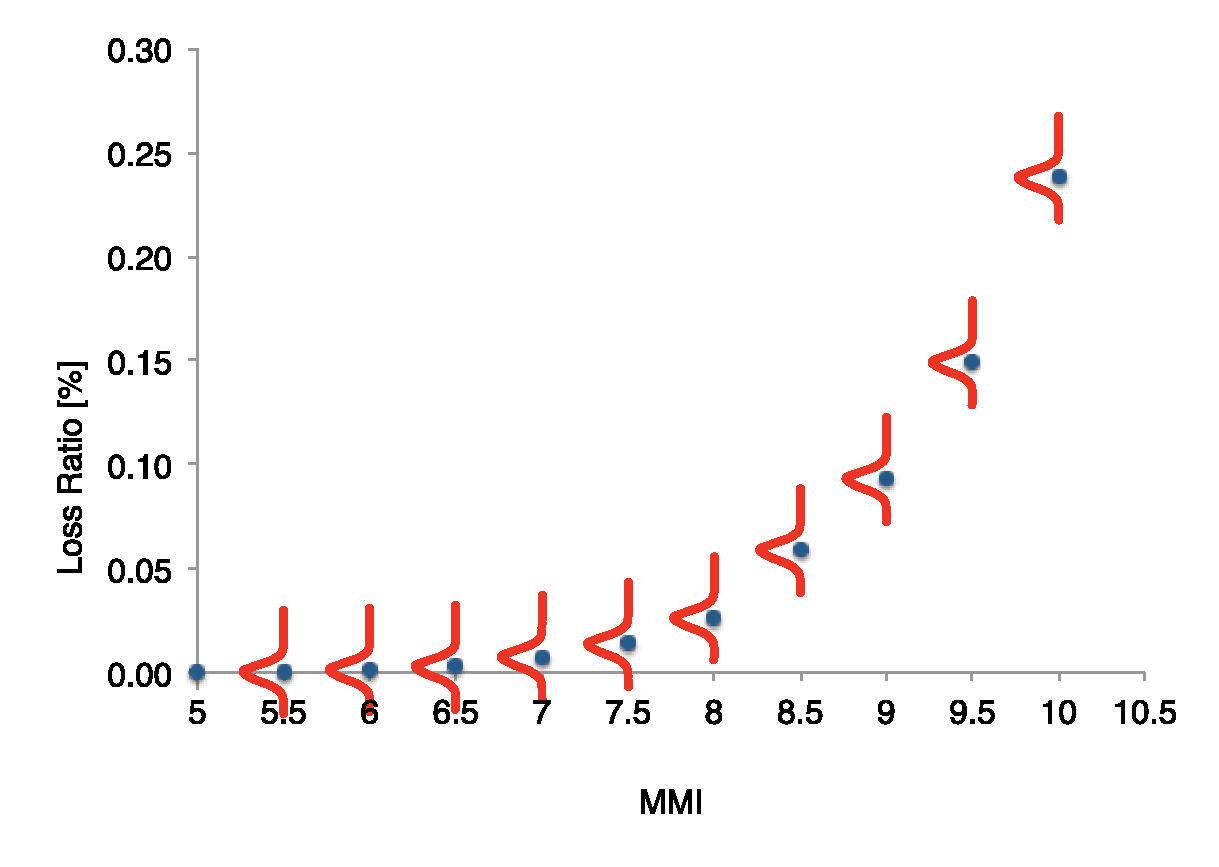
\includegraphics[width=10cm,height=6cm]{./figures/risk/VFDiscrete.eps}
\caption{Discrete vulnerability function.}
\label{fig:VFDiscrete}
\end{figure}

\color{blue}
\subsubsection{Continuous Vulnerability Functions}
\index{Physical Vulnerability!Continuous Functions}
\marginpar{Continuous vulnerability functions are not currently supported}
Continuous \glspl{vulnerability function} may be implemented in future versions of the OpenQuake engine. Continuous \glspl{vulnerability function} will probably be described by continuous distributions of mean loss ratio and other fractiles of loss ratio, with ground motion intensity. Figure \ref{fig:VFContinuous} illustrates this type of function, showing the distribution of mean loss and the 10 percent and 90 percent fractiles.

\begin{figure}[ht]
\centering
\includegraphics[width=10cm,height=6cm]{./figures/risk/VFContinuous}
\caption{Continuous vulnerability function.}
\label{fig:VFContinuous}
\end{figure}
\color{black}

\subsection{Fragility Functions}
\index{Fragility}
\Glspl{fragility function} describe the probability of exceeding a set of limit states, given an intensity measure level. When the asset category concerns structures (e.g. buildings), the intensity measure can either be structure-independent or structure-dependent. The former can be calculated directly from recorded measurements of ground shaking (e.g. peak ground acceleration, peak ground velocity, spectral acceleration at a given period of vibration, or even macroseismic intensity). The latter requires information on the characteristics of the structures in order to be calculated, for example spectral acceleration at the fundamental period of vibration, or spectral displacement at the limit state period of vibration. The calculation of these structural characteristics might be through a simple formulae (e.g. a yield period-height equation, see e.g. \citet{CrowleyPinho2004} ) or through so-called non-linear static methods, which are needed when the intensity measure is a non-linear response quantity such as spectral displacement at the limit state period of vibration (see e.g. \citet{FEMA440ATC2005}). The oq-risklib currently does not support non-linear static methods.

\subsubsection{Discrete Fragility Functions}
\index{Fragility!Discrete Functions}
\Glspl{fragility function} can be defined in a discrete way by providing, for each limit state, a list of intensity measure levels and respective probabilities of exceedance. Figure \ref{fig:FFDiscrete} presents a set of discrete \glspl{fragility function} using a macroseismic intensity measure. 

\begin{figure}[ht]
\centering
\includegraphics[width=10cm,height=6cm]{./figures/risk/FFDiscrete.eps}
\caption{Set of discrete fragility functions.}
\label{fig:FFDiscrete}
\end{figure}

\subsubsection{Continuous Fragility Functions}
\index{Fragility!Continuous Functions}
Continuous \glspl{fragility function} are defined by the parameters of a cumulative distribution function. In Figure \ref{fig:FFcontinuous} an example of a set of continuous fragility functions with a structure-dependent intensity measure is presented. 

\begin{figure}[ht]
\centering
\includegraphics[width=10cm,height=6cm]{./figures/risk/FFContinuous.eps}
\caption{Set of continuous fragility functions.}
\label{fig:FFcontinuous}
\end{figure}

\color{blue}
\subsubsection{Uncertainty in Fragility Functions}
\index{Fragility!Uncertainty}
\marginpar{uncertainty in fragility functions is not currently supported}
The uncertainty in continuous glspl{fragility function} will be accounted for in future versions of the engine. Figure \ref{fig:FF_uncertainty} shows a lognormal distribution that has been fit to the data (i.e. the fragility function), and the probabilistic distribution (i.e. mean and standard deviation) to describe the uncertainty in both the logarithmic mean and logarithmic standard deviation of the fragility function. When a set of glspl{fragility function} for different limit states are used, it is also necessary to provide information on the correlation between the logarithmic means and logarithmic standard deviations of each limit state.

\begin{figure}[ht]
\centering
\includegraphics[width=12cm,height=6cm]{./figures/risk/FFuncertainty.eps}
\caption{Uncertainty of continuous fragility functions.}
\label{fig:FF_uncertainty}
\end{figure}


\subsection{Consequence Functions}
\index{Consequence Functions}
\marginpar{Consequence functions are not currently supported}
\Glspl{consequence function} describe the probability distribution of loss, given a performance level. For example, if the asset category is buildings and the performance level is significant damage, the \gls{consequence function} will describe the mean loss ratio, coefficient of variation and probability distribution for that level of damage. Figure \ref{fig:ConsequenceFunctions} presents the mean damage ratios for a set of performance levels proposed by two different sources. Although these functions are not directly supported, users can combine \glspl{consequence function} with \glspl{fragility function} to produce \glspl{vulnerability function} to be input into the engine.  

\begin{figure}[Ht]
\centering
\includegraphics[width=10cm,height=6cm]{./figures/risk/ConsequenceFunction.eps}
\caption{Consequence functions adapted from  \citet{Baletal2010}}
\label{fig:ConsequenceFunctions}
\end{figure}
\color{black}

% ------------------------------------------------------------------------------
\chapter{Scenario Risk Calculator}
	\label{chap:scenario_risk}
	

\section{Introduction}
\index{Scenario Risk}
The scenario risk calculator is capable of computing losses and loss statistics from a single event for a collection of assets, given a set of \glspl{groundmotionfield}. The use of a set of \glspl{groundmotionfield} is recommended so that the aleatory variability (both inter- and intra-event) in the \gls{groundmotionpredictioneq} is modelled. The input \glspl{groundmotionfield} can be calculated with oq-hazardlib or by an external software; in either case they need to be stored in the OpenQuake engine database. With the use of the oq-hazardlib, these \glspl{groundmotionfield} can be calculated either with or without the spatial correlation of the ground motion residuals.

For each \gls{groundmotionfield}, the intensity measure level at a given site is combined with a \gls{vulnerability function}, from which a loss ratio is randomly sampled, for each \gls{asset} contained in the \gls{exposure model}. The loss ratios that are sampled for \glspl{asset} of a given \gls{taxonomy} classification at different locations can be considered to be either independent, fully correlated, or correlated with a specific correlation coefficient. Using these results, the mean and standard deviation of the loss ratios across all \glspl{groundmotionfield} can be calculated. Loss ratios are converted into \gls{groundupLosses} by multiplying by the cost (which can be the structural, non-structural or contents) of the \gls{asset} given in the exposure model. It is furthermore possible to sum the losses throughout the region and to compute the mean and standard deviation of the total loss. This process is common to any of the costs type (structural, non-structural or contents) or occupants.
Besides the \gls{groundupLosses}, it is also possible to calculate \gls{insuredLosses} (i.e. economic value that can be covered by the insurance industry according to a certain policy). To do so, both a \gls{deductible} and a \gls{limit} for each type of cost (structural, non-structural or contents) need to be defined. The methodologies employed to calculate the \gls{groundupLosses} and \gls{insuredLosses} are described below.

\section{Calculation Steps}

To compute the mean \gls{groundupLosses}:

\begin{enumerate}
\item For each \gls{groundmotionfield}, the intensity measure level at the location of the \gls{asset} is used to derive the mean loss ratio and associated coefficient of variation from the \gls{vulnerability function}. Since currently the \glspl{vulnerability function} are being defined in a discrete manner, it is quite probable that the intensity measure level provided by the \gls{groundmotionfield} is not contained in the \gls{vulnerability function}. In these cases, linear interpolation methods are being employed to derive the mean loss ratio at the intensity measure level of interest. 

\item The engine takes the \gls{vulnerability function} assigned to each \gls{asset} and checks if the coefficient of variation is zero. If so, the loss ratios are derived based on the mean loss ratio for each intensity measure level. Otherwise, if the uncertainty is defined, it is randomly sampled following the probabilistic distribution of the respective \gls{vulnerability function}, as described below:

\begin{equation}
\log{LR_n} = \mu + \epsilon\sigma
\end{equation}

Where $\mu$ and $\sigma$ stand for the mean and standard deviation of the logarithm of the loss ratios, respectively, and $\epsilon$ is a term that has a standard normal distribution with a zero mean and a standard deviation of one.  

The method used to sample epsilon depends on whether the correlation between the vulnerability uncertainty of \glspl{asset} of a given \gls{taxonomy} is to be considered or not:

\begin{itemize}

\item Perfectly correlated: the term $\epsilon$ is randomly sampled once for the first \gls{asset} and this result is used to derive the loss ratio for all the \glspl{asset} of the same \gls{taxonomy}. 

\item Correlated: the term $\epsilon$ is randomly sampled for each \gls{asset} considering the specified correlation coefficient between \glspl{asset}. 

\item Uncorrelated: the term $\epsilon$ is always randomly sampled for each \gls{asset} and therefore the correlation between the vulnerability of the \glspl{asset} is ignored.

\end{itemize}

\item The mean loss ratio for each \gls{asset} across all possible simulations of the scenario event can be calculated through the formula:

\begin{equation}
LR=\frac{\sum^m_{n=1}LR_n|IML}{m}
\end{equation}

Where $m$ stands for the number of ground motion fields simulated.

\item The mean loss can then be derived by multiplying the mean loss ratio by the value of the \gls{asset} contained in the \gls{exposure model} file.

\end{enumerate}

To compute the standard deviation of the ground-up losses:

\begin{enumerate}

\item In order to compute the uncertainty, the engine takes the set of loss ratios for each \gls{asset}, and computes the associated standard deviation using the classical formula:

\begin{equation}
SD[LR]=\sqrt{  \frac{1}{m}\sum_{n=1}^m{(LR_n-E[LR])^2} }
\end{equation}

Where $E[LR]$ stands for the mean loss ratio computed previously.

\item The standard deviation of the absolute loss can finally be computed by multiplying the standard deviation of the loss ratio by the value of the respective \gls{asset}.

\end{enumerate}

To compute the \gls{insuredLosses}:
The calculation of the insured losses is valid for the structural, non-structural and contents costs. When the computation of the insured losses is triggered, the ground-up losses from each asset, at each \gls{groundmotionfield} are modified in the following manner:

\begin{enumerate}

\item If the limit has been defined in a relative way, this fraction is first multiplied by the respective total cost, in order to obtain the absolute value. If the ground-up loss is above the absolute limit, the resulting loss is reduced to this threshold.

\item Then, the absolute deductible is taken directly from the exposure model, or calculated by multiplying the associated fraction by the respective total cost. Once the absolute deductible is obtained, the ground-up loss is further reduced by this amount. If the deductible is above the ground-up loss, then the insured loss is null.

This process is clarified in Figure \ref{fig:insuredLosses}.

\begin{figure}[ht]
\centering
\includegraphics[width=14cm,height=7cm]{./figures/risk/insuredLosses.eps}
\caption{Representation of the process to estimate the insured losses.}
\label{fig:insuredLosses}
\end{figure} 

In Case A, the ground-up loss does not exceed the deductible, which leads to an insured loss equal to zero. In Case B, the ground-up loss is above the deductible, but does not reach the limit. Hence, the resulting insured loss if equal to the ground-up loss minus the deductible. Finally, in Case C the ground up loss is greater than the limit. Thus, this loss is firstly reduced to the value of the limit, and then  the deductible is subtracted. In other words, the portion of the ground-up losses that are insured, is the fraction located between the deductible and the limit thresholds.   

\item The calculation of the mean and standard deviation of the insured losses follows the same approach described previously for the ground-up losses.

\end{enumerate}

\section{Calculator Output}
The output of the Scenario Risk Calculator currently comprises ground-up and insured loss statistics (mean total loss and standard deviation of total loss) and ground-up and insured loss maps. Loss maps are comprised by a set of loss nodes, which are associated with a pair of coordinates. For each node, one or more loss values might exist, due to the fact that several different \glspl{asset} can be located at the same location.  Figure \ref{fig:detlosses} presents an example of a loss map containing the expected economic losses for residental buildings located in Nepal, considering a rupture of magnitude 7.0Mw in the central part of the country.

\begin{figure}[ht]
\centering
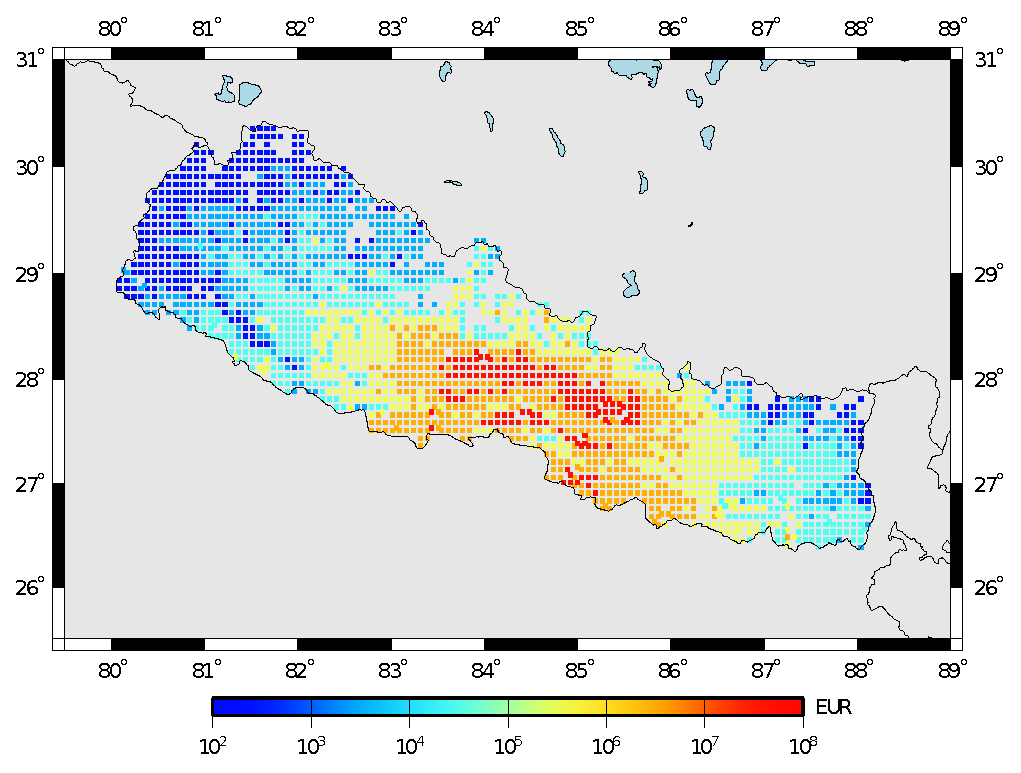
\includegraphics[width=12cm,height=8cm]{./figures/risk/LossmapDet.eps}
\caption{Loss map with the distribution of mean economic losses for residential buildings in Nepal.}
\label{fig:detlosses}
\end{figure} 
% ------------------------------------------------------------------------------
\chapter{Scenario Damage Calculator}
	\label{chap:scenario_damage}
	

\section{Introduction}
\index{Scenario Damage}
The scenario damage calculator can be employed to estimate the distribution of damage due to a single earthquake, for a spatially distributed building portfolio. Similarly to what has been described for the scenario risk calculator, a finite \gls{rupture} should be used to derive sets of \glspl{groundmotionfield}. 

In this calculator, each \gls{groundmotionfield} is combined with a \gls{fragility model} (discrete or continuous), in order to compute the fractions of buildings in each damage state. These fractions are calculated based on the difference in probabilities of exceedance between consecutive limit state curves at a given intensity measure level. This process is repeated for each \gls{groundmotionfield}, leading to a list of fractions for each \gls{asset}. These results can then be multiplied by the respective number or area of buildings in order to obtain the absolute building damage distribution.

\section{Calculation Steps}

\begin{enumerate}
\item For each \gls{groundmotionfield}, the intensity measure level at the location of the \gls{asset} is used to derive the
fraction of buildings in each damage state. In order to do so, the distance between each pair of consecutive limit states is calculated. This process is illustrated in Figure \ref{fig:FragilityProcess}, using a continuous \gls{fragility function}.

\begin{figure}[ht]
\centering
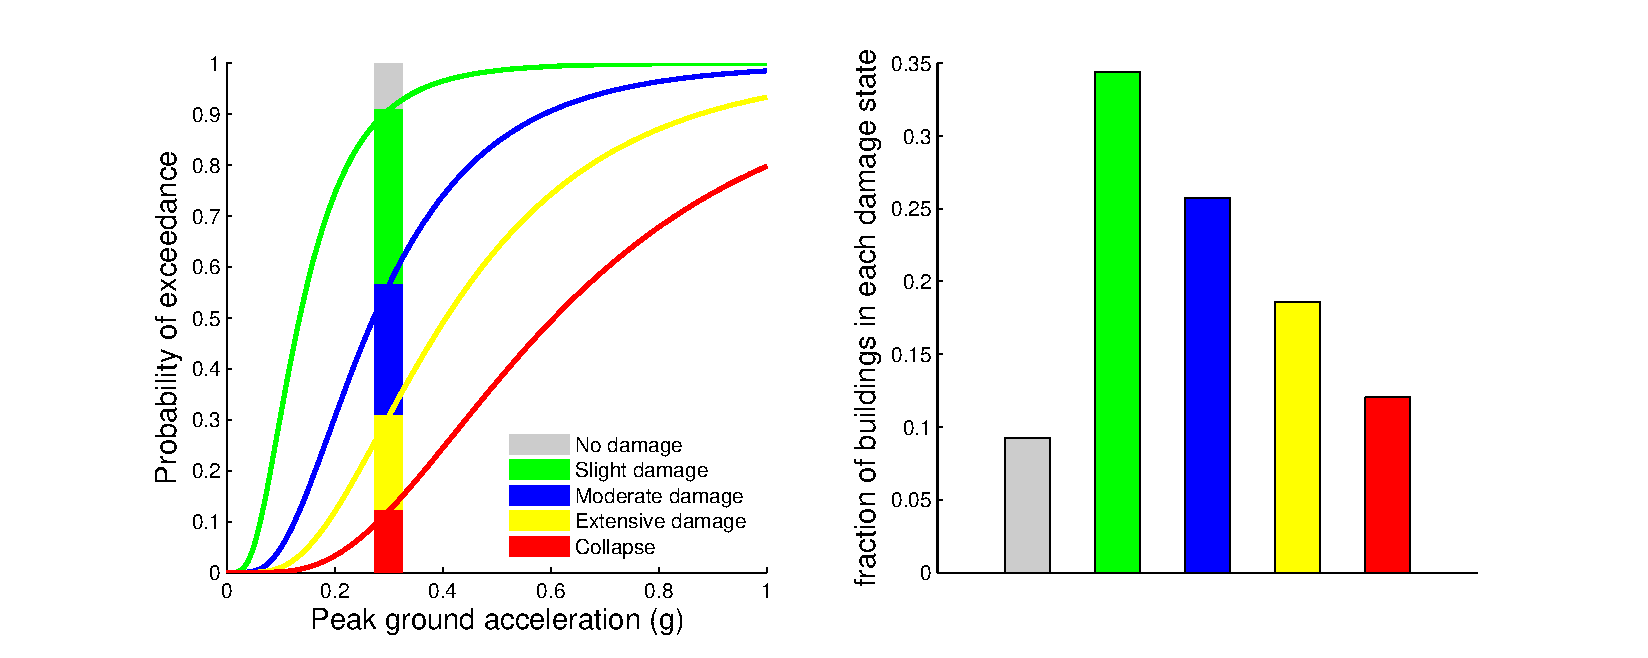
\includegraphics[width=14cm,height=5cm]{./figures/risk/Fragility_process.eps}
\caption{Representation of the fractions of building in each damage states, for a given intensity measure level (0.3 g).}
\label{fig:FragilityProcess}
\end{figure}

When a continuous \gls{fragility function} is used for the calculations, the fractions of building in each damage state are calculated using the analytical expression of the lognormal cumulative distribution functions. On the other hand, if a discrete \gls{fragility function} was chosen, these fractions are computed using linear interpolation between the pair of points either side of the intensity measure level.

\item Step 1 is repeated for each \gls{groundmotionfield}, leading to a list of fractions (one per damage state), for each \gls{asset}. From this list of values, the mean ($E[FR]$) and standard deviation ($SD[FR]$) for each fraction can be estimated using the following formulae:

\begin{equation}
E[FR]=\frac{\sum^m_{n=1}FR_n|IML}{m}
\end{equation}

\begin{equation}
SD[FR]=\sqrt{  \frac{1}{m}\sum_{n=1}^m{(FR_n-E[FR])^2} }
\end{equation}
 
Where $m$ stands for the number of \glspl{groundmotionfield} simulated. 

\item These fractions of buildings in each damage state can be multiplied by the quantity of the respective asset, leading to the mean and standard deviation of the number or area of buildings in each damage state (see Figure \ref{fig:AssetDis}). 

\item This calculator is also capable of estimating the aggregated number or area of buildings from the same \gls{taxonomy} in each damage state (see Figure \ref{fig:TaxDis}). In order to do so, for each \gls{groundmotionfield}, the absolute quantity of buildings in each damage state is calculated, and aggregated according to their \gls{taxonomy}. After processing all the \glspl{groundmotionfield}, the associated statistics for each building \gls{taxonomy} are calculated according to the formulae described in Step 2.

\item The total damage distribution is also calculated, by summing the quantity of buildings in each damage state, across all the \glspl{asset} existing in the building portfolio. This calculation will lead to a single damage distribution, represented by a mean and standard deviation for each damage state (see Figure \ref{fig:TotalDis}).

\end{enumerate}

\section{Calculator Output}
The output of the Scenario Damage Calculator currently comprises damage distributions at three levels: per \gls{asset}, per building \gls{taxonomy} and total. In addition, with this calculator, it is also possible to extract collapse maps, which contain the spatial distribution of the number or area of collapsed buildings throughout the region of interest (see Figure \ref{fig:CollapseMap}). In the figures shown herein, examples of the outputs are depicted for a scenario event of magnitude 7.0Mw in the central region of Nepal.

\begin{figure}[ht]
\centering
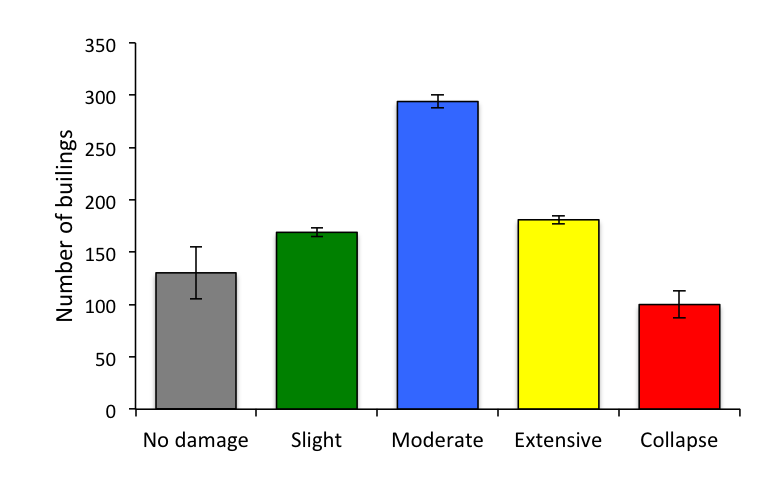
\includegraphics[width=8cm,height=5cm]{./figures/risk/AssetDisaggregation.eps}
\caption{Damage distribution for a single asset.}
\label{fig:AssetDis}
\end{figure} 

\begin{figure}[ht]
\centering
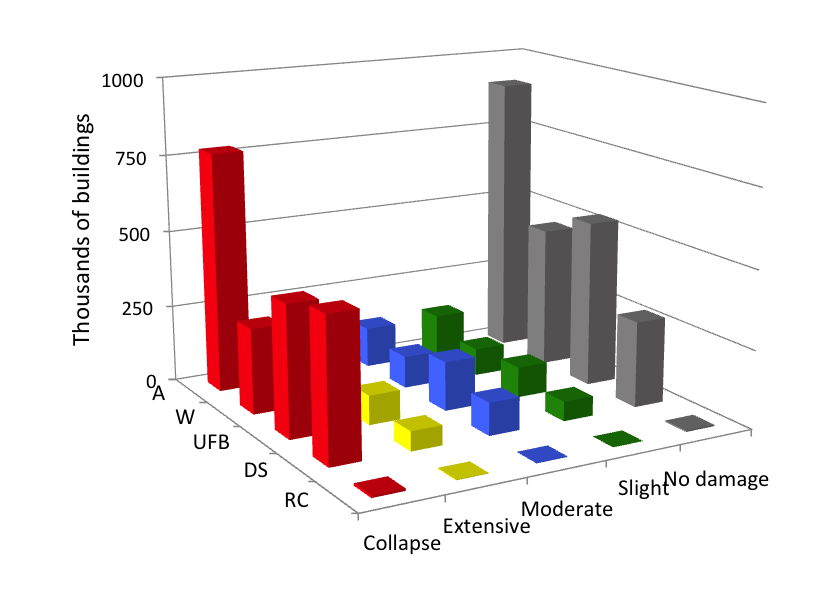
\includegraphics[width=8cm,height=5cm]{./figures/risk/TaxonomyDisaggregation.eps}
\caption{Damage distribution according to the building taxonomy.}
\label{fig:TaxDis}
\end{figure} 

\begin{figure}[ht]
\centering
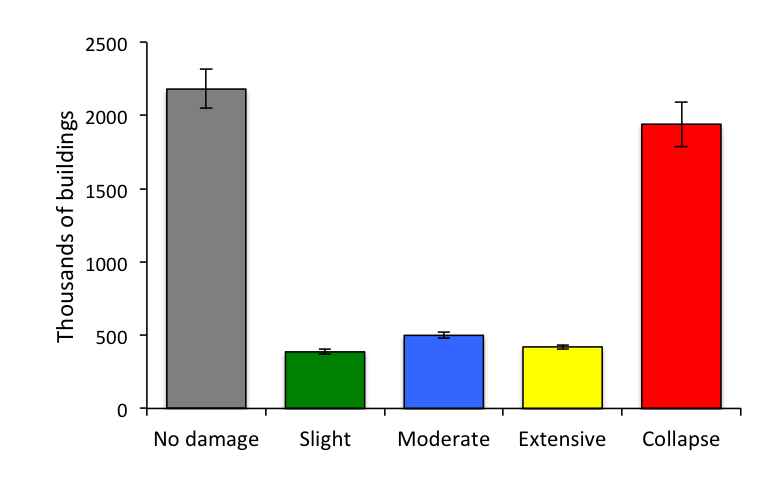
\includegraphics[width=8cm,height=5cm]{./figures/risk/TotalDis.eps}
\caption{Damage distribution of the whole building portfolio.}
\label{fig:TotalDis}
\end{figure} 

\begin{figure}[ht]
\centering
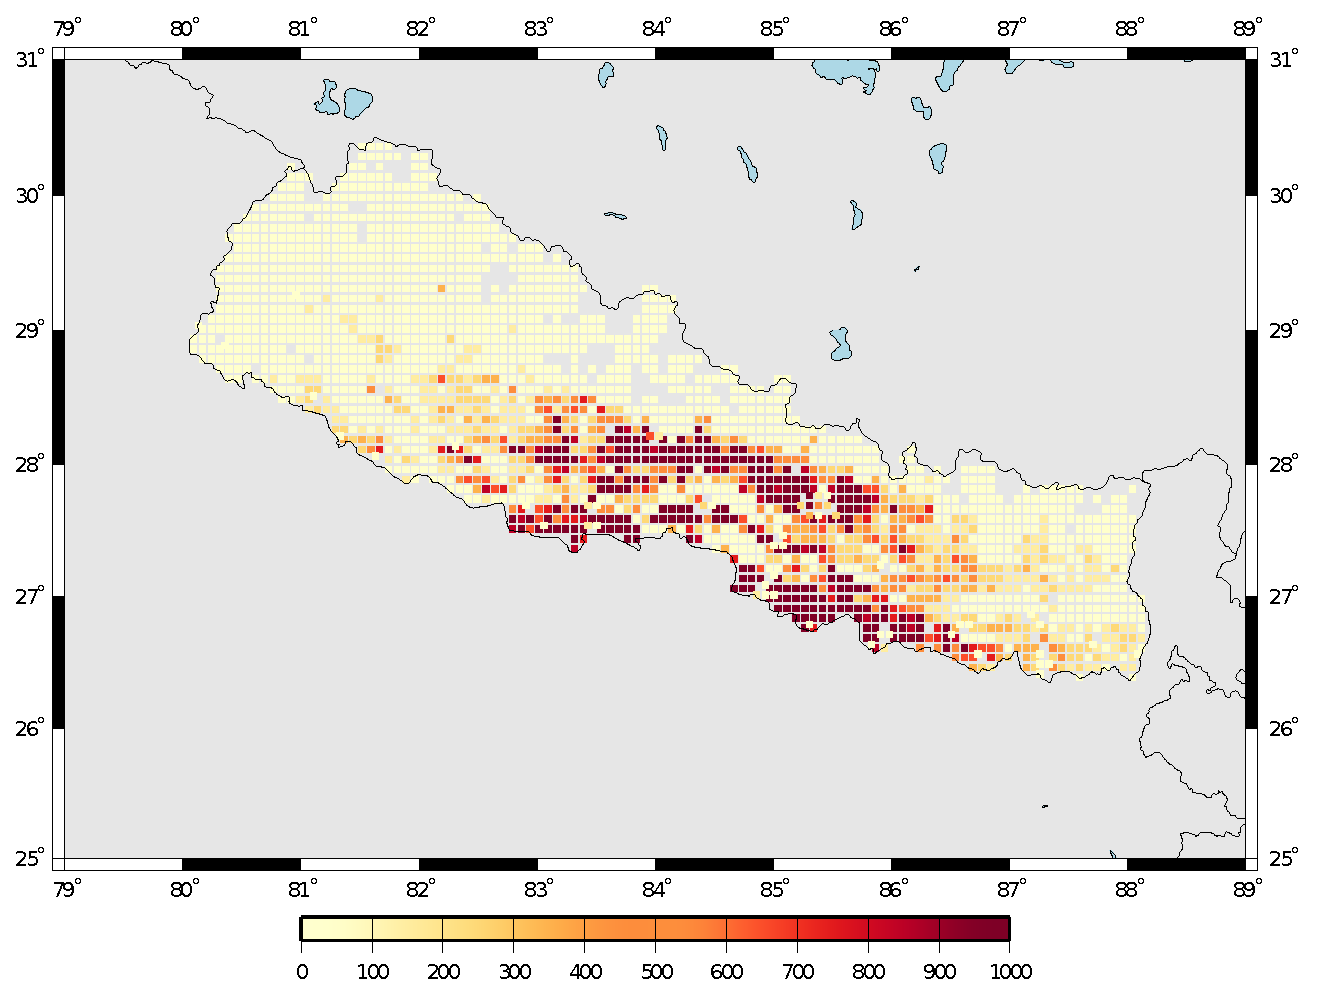
\includegraphics[width=12cm,height=8cm]{./figures/risk/CollapseMap.eps}
\caption{Collapse map considering the whole building portfolio.}
\label{fig:CollapseMap}
\end{figure} 
% ------------------------------------------------------------------------------
\chapter{Probabilistic Event-Based Risk Calculator}
	\label{chap:risk_prob_event_based}
	\section{Introduction}
\index{Probabilistic Risk!Event-Based}
The probabilistic event-based risk calculator uses \glspl{stochasticeventset} and associated \glspl{groundmotionfield} to compute loss exceedance curves for each \gls{asset} contained in an \gls{exposure model}. This calculator thus requires \glspl{groundmotionfield} from a number of stochastic events as an input, which the engine can calculate using the oq-hazardlib.

For each \glspl{groundmotionfield}, the intensity measure level at a given site is combined with a \gls{vulnerability function}, from which a loss ratio is randomly sampled, for each \gls{asset} contained in the \gls{exposure model}. The loss ratios that are sampled for \glspl{asset} of a given \gls{taxonomy} classification at different locations are considered to be either independent or correlated. The losses for a given asset are calculated using all of the \glspl{groundmotionfield}, leading to list of events and associated loss ratios. This list is then sorted from the highest loss ratio to the lowest. The rate of exceedance of each loss ratio is calculated by dividing the number of exceedances of that loss ratio by the number of \glspl{stochasticeventset} multiplied by the length of each event set. By assuming a Poissionian distribution of the occurrence model, the probability of exceedance of each loss ratio is calculated. If a total loss curve for a portfolio of \glspl{asset} is required, a secondary module is used in order to sum the losses from all the \glspl{asset} in the exposure file, per event, before calculating the exceedance distribution of loss. This distribution of the total losses per event can also be extracted, and it is termed here as an \gls{eventLossTable}.

Similarly to what has been described for the Scenario Risk Calculator (see section \ref{chap:scenario_risk}), this module can compute \gls{insuredLosses} following the same approach (i.e. modifying the  loss based on the \gls{deductible} and \gls{limit} for each cost type).

This calculator is also capable of performing \gls{lossdisaggregation} in terms of magnitude/distance or latitude/longitude. In order to do so, the losses at each location are disaggregated based on the aforementioned parameters, and a loss percentage for each possible combination is calculated.

\section{Calculation Steps}

To compute the loss exceedance curves:

\begin{enumerate}
\item The oq-engine starts by using the set of \glspl{groundmotionfield} to extract the intensity measure levels for the location of each \gls{asset}. 
 
\item Then the oq-engine takes the \gls{vulnerability function} assigned to each \gls{asset} and checks if the coefficient of variation is zero. If so, the loss ratios are derived based on the mean loss ratio for each intensity measure level. Otherwise, if the uncertainty is defined, it is randomly sampled following the probabilistic distribution, mean loss ratio and associated coefficient of variation of the respective function, as described below:

\begin{equation}
\log{LR_n} = \mu + \epsilon\sigma
\end{equation}

Where $\mu$ and $\sigma$ stand for the mean and standard deviation of the logarithm of the loss ratios respectively and $\epsilon$ is a term that has a standard normal distribution with a zero mean and a standard deviation of one.  

The method used to sample epsilon can follow tree approaches depending on whether the correlation between the vulnerability of \glspl{asset} of a given \gls{taxonomy} is to be considered or not:

\begin{itemize}

\item Perfectly correlated: the term $\epsilon$ is randomly sampled once for the first \gls{asset} and this result is used to derive the loss ratio for all the \glspl{asset} of the same \gls{taxonomy}. 

\item Correlated: the term $\epsilon$ is randomly sampled for each \gls{asset} considering the specified correlation coefficient between \glspl{asset}. 

\item Uncorrelated: the term $\epsilon$ is always randomly sampled for each \gls{asset} and therefore the correlation between the vulnerability of the \glspl{asset} is ignored.
\end{itemize}

\item Each loss ratio is multiplied by the associated asset value, leading to the absolute loss values. If these losses are related with the structural, non-structural or contents cost, the \gls{insuredLosses} module can be used to modify the \gls{groundupLosses} according to the associated \gls{deductible} and \gls{limit} thresholds, as described in section \ref{chap:scenario_risk}.

\item In this method the losses to each \gls{asset} for each event are estimated and then sorted from highest to lowest. The rate of exceedance of each loss is calculated by dividing the number of exceedances of that loss by the number of \glspl{stochasticeventset} multiplied by the length of each event set. Hence, the top loss will have zero exceedances, the next loss ratio will have one exceedance, and so on.

The following formula is employed to compute the rate of exceedance:

\begin{equation}
\lambda(L_n) = \frac{NE_{L}}{TSES}
\end{equation}

Where  $\lambda$ stands for the rate of exceedance of the respective loss ratio, $NE_{L}$ stands for the number of exceedances of the given loss, and $TSES$ stands for the time span of all \glspl{stochasticeventset}, i.e. the number of \glspl{stochasticeventset} multiplied by the time span of each.

\item Assuming a Poissonion distribution of the occurrence model, the probability of exceedance of the set of losses in a given time span can be derived using the following formula:

\begin{equation}
PE(L_n) = 1-\exp{-\lambda_n\times t}
\end{equation}

Where $t$ stands for the time span used to produce the \gls{stochasticeventset}.

\end{enumerate}

To perform the loss disaggregation:

\begin{enumerate}

\item For the disaggregation of the losses it is necessary to provide the coordinates of the locations where this procedure should be employed. Then, for the selected locations, the oq-engine calculates the sum of the losses (considering all the assets existing at each of the selected sites) for each seismic event. In addition, the rupture distance (Joyner-Boore) and coordinates of the point within the vertical projection of the rupture plane closest to each site are estimated. An example of this type of information is presented in Figure \ref{fig:SetLosses}, for 20 stochastically produced seismic events.

\begin{figure}[ht]
\centering
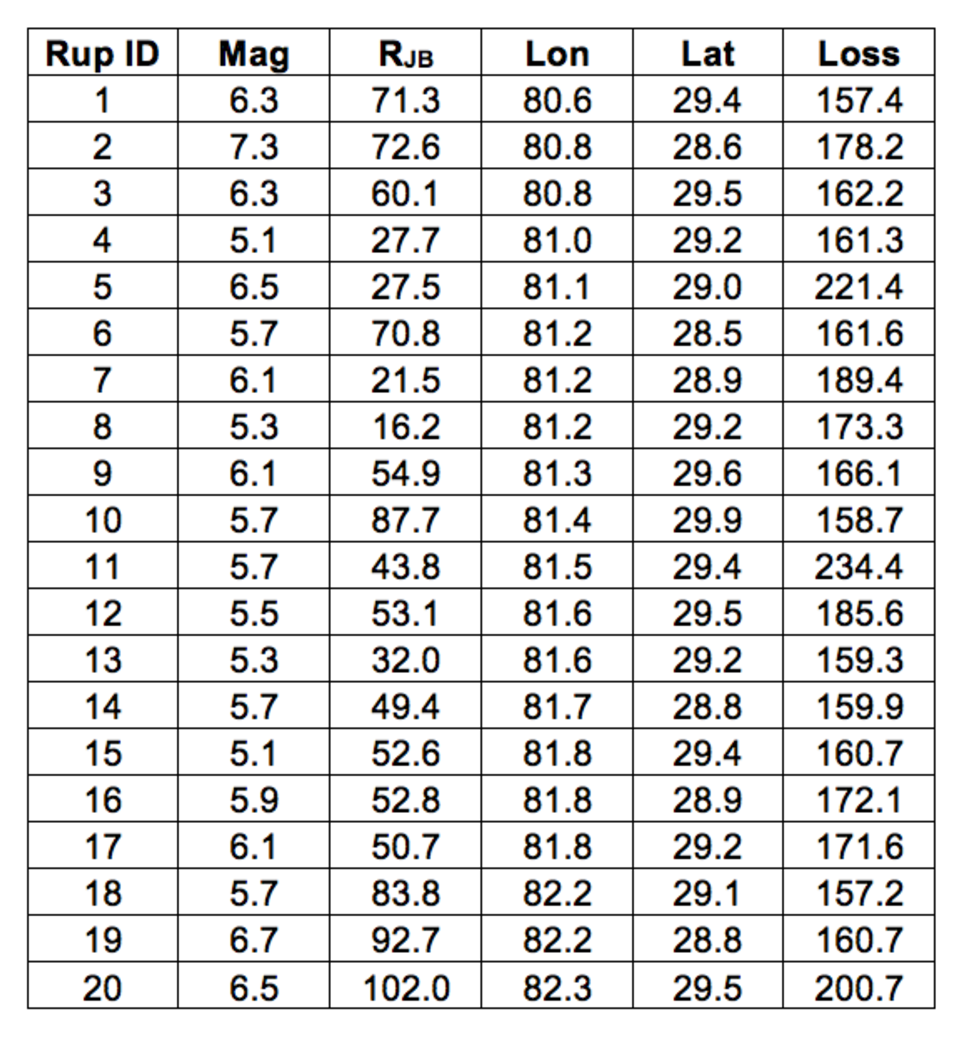
\includegraphics[width=9cm,height=10cm]{./figures/risk/SetLosses.eps} 
\caption{Economic losses from a single asset for a set of seismic events.}
\label{fig:SetLosses}
\end{figure} 

\item The oq-engine calculates the range (maximum and minimum values) of the list of magnitudes, distances, latitudes and longitudes across all the events, and using the increment defined for each parameter, a set of linearly spaced bins is calculated. Then, the losses from every seismic event are aggregated depending into which combination of magnitude/distance or latitude/longitude they fall. The previously presented losses have been disaggregated according to these two combinations as presented in Figure \ref{fig:Dis}:

\begin{figure}[ht]
\centering
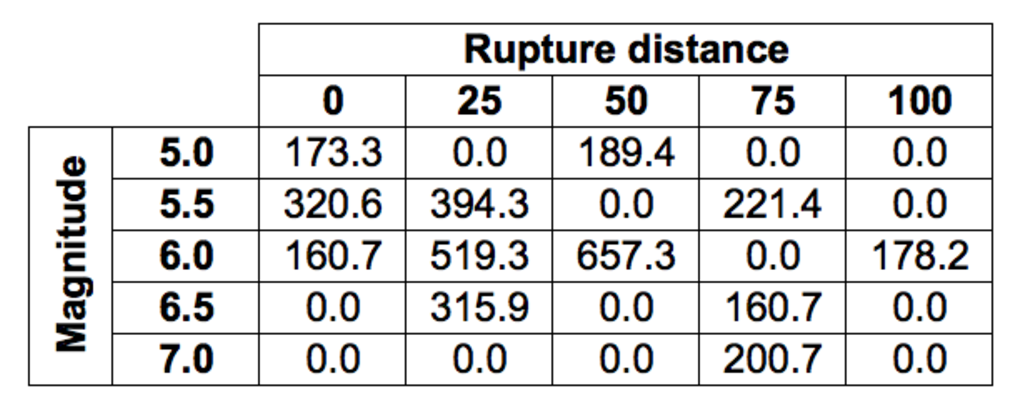
\includegraphics[width=8cm,height=3cm]{./figures/risk/DisaggregationDistMag.eps} 
\includegraphics[width=8cm,height=2.8cm]{./figures/risk/DisaggregationCoor.eps} 
\caption{Disaggregation of the economic losses according to a set of magnitude/distance and latitude/longitude combinations.}
\label{fig:Dis}
\end{figure} 

\item The resulting losses for each pair of parameters (magnitude/distance and latitude/longitude) are divided by the total loss across all the events. This percentage of the overall loss for each combination is depicted in Figure \ref{fig:disaggregation} in the following section.
\end{enumerate}

\section{Calculator Output}
The output of this calculator comprises loss exceedance curves and loss maps. Loss exceedance curves are represented by a list of losses and respective probabilities of exceedance. Furthermore, each curve is associated with a pair of coordinates, an end branch label (that allows the curve to be connected to the set of specifications used in the calculations) and an asset ID (that permits tracking of the asset that each loss curve was computed for). Loss maps for a given probability of exceedance in a given time span can be produced, as well as maps of mean loss within a given time span. Figure \ref{fig:LossCurve01} and \ref{fig:LossCurve001} present a loss map for a probability of exceedance of 1\% and 10\% in 50 years for residential buildings located in Nepal, respectively. 

\begin{figure}[H]
\centering
\includegraphics[width=12cm,height=8cm]{./figures/risk/LossMap01.eps} 
\caption{Loss map for a probability of exceedance of 10\% in 50 years.}
\label{fig:LossCurve001}
\end{figure} 

\begin{figure}[H]
\centering
\includegraphics[width=12cm,height=8cm]{./figures/risk/LossMap001.eps} 
\caption{Loss map for a probability of exceedance of 1\% in 50 years.}
\label{fig:LossCurve01}
\end{figure} 

For this calculator, total loss exceedance curves can be produced which combine the losses to all \glspl{asset} per event. It is noted that loss exceedance curves which present the probability of exceedance of the aggregate annual losses, or maximum annual losses, are not yet supported in the oq-risklib. In Figure \ref{fig:ProbLosses}, a total loss exceedance curve for the residential building portfolio in Nepal is presented. 
 
\begin{figure}[H!]
\centering
\includegraphics[width=8cm,height=6cm]{./figures/risk/LossCurveIstanbul.eps}
\caption{Total loss exceedance curve for RC buildings.}
\label{fig:ProbLosses}
\end{figure} 

For what concerns the \glspl{eventLossTable}, the oq-engine can extract the total loss across all the assets for each seismic event. The results is a table with the rupture id, magnitude and total loss, as illustrated in Figure \ref{fig:eventLossTable}.

\begin{figure}[H!]
\centering
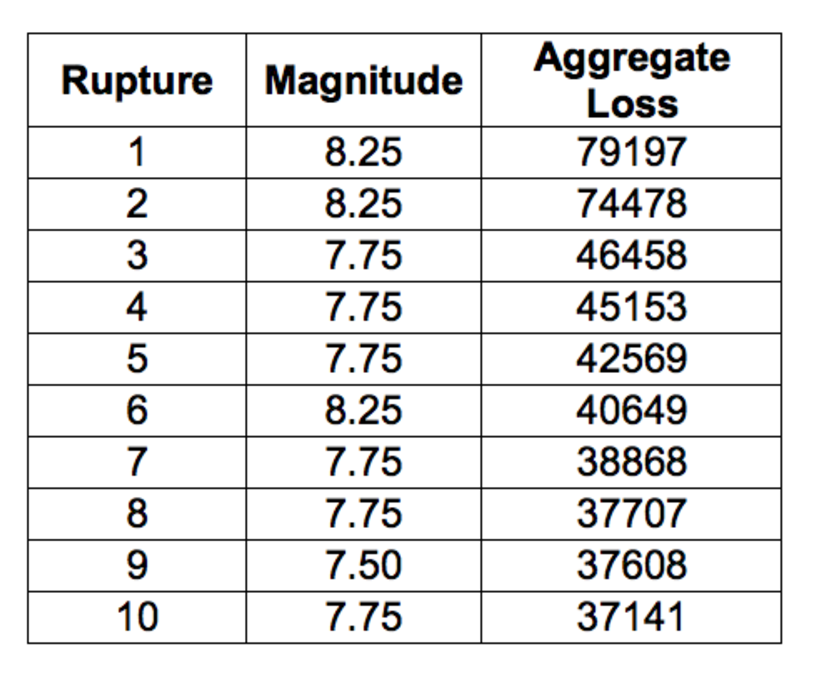
\includegraphics[width=6cm,height=5cm]{./figures/risk/EventLossTable.eps}
\caption{Example of an \gls{eventLossTable}.}
\label{fig:eventLossTable}
\end{figure} 

The output of the \gls{lossdisaggregation} is composed by the loss fraction associated to each combination of parameters (magnitude/distance or latitude/longitude), as presented in Figure \ref{fig:disaggregation} .

\begin{figure}[H!]
\centering
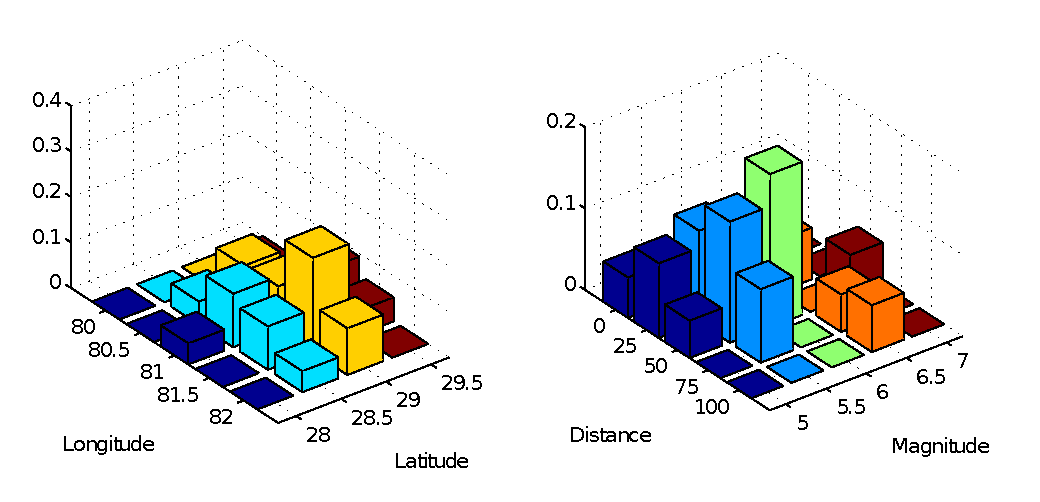
\includegraphics[width=14cm,height=6.5cm]{./figures/risk/Disaggregation.eps}
\caption{Example of a loss disaggregation according to a set of magnitude/distance and latitude/longitude combinations.}
\label{fig:disaggregation}
\end{figure} 

% ------------------------------------------------------------------------------
\chapter{Classical PSHA-Based Risk Calculator}
	\label{chap:risk_psha_based}
	\input{./oqbr/Classical_PSHA_Based.tex}
% ------------------------------------------------------------------------------
\chapter{Retrofitting Benefit/Cost Ratio Calculator}
	\label{chap:bcr}
	\section{Introduction}
\index{Benefit/Cost Ratio}

The retrofitting benefit/cost ratio calculator allows users to understand if from an economical point of view, a collection of buildings should be retrofitted. This calculator uses loss exceedance curves that can be calculated using either the probabilistic event-based risk or the classical PSHA-based risk calculators (see Figure \ref{fig:Scheme_bcr_calc}). These curves need to be calculated considering two \glspl{vulnerability model}: one with the original asset vulnerability, and a second one using the retrofitted vulnerability configuration. The average annual ground-up losses considering both vulnerability configurations are calculated, and employed to estimate the economic saving during the life expectancy (or design life) of the \glspl{asset}. This benefit is divided by the retrofitting cost, thus obtaining the benefit/cost ratio. This ratio is modified considering the inflation rate to take into account the fact that the losses will be observed in the future, whereas the cost is outlayed today. A ratio above one indicates that a retrofitting intervention would be advantageous from an economic point of view.

\section{Calculation Steps}

\begin{enumerate}
\item This calculator starts by calculating loss exceedance curves for a collection of \glspl{asset}, using either the classical PSHA-based risk calculator or the probabilistic event-based risk calculators. Two configurations of the vulnerability need to be considered: original and retrofitted. Thus, for each \gls{asset}, two loss exccedance curves are determined, as depicted in Figure \ref{fig:VulLosscurve}.

\begin{figure}[ht]
\centering
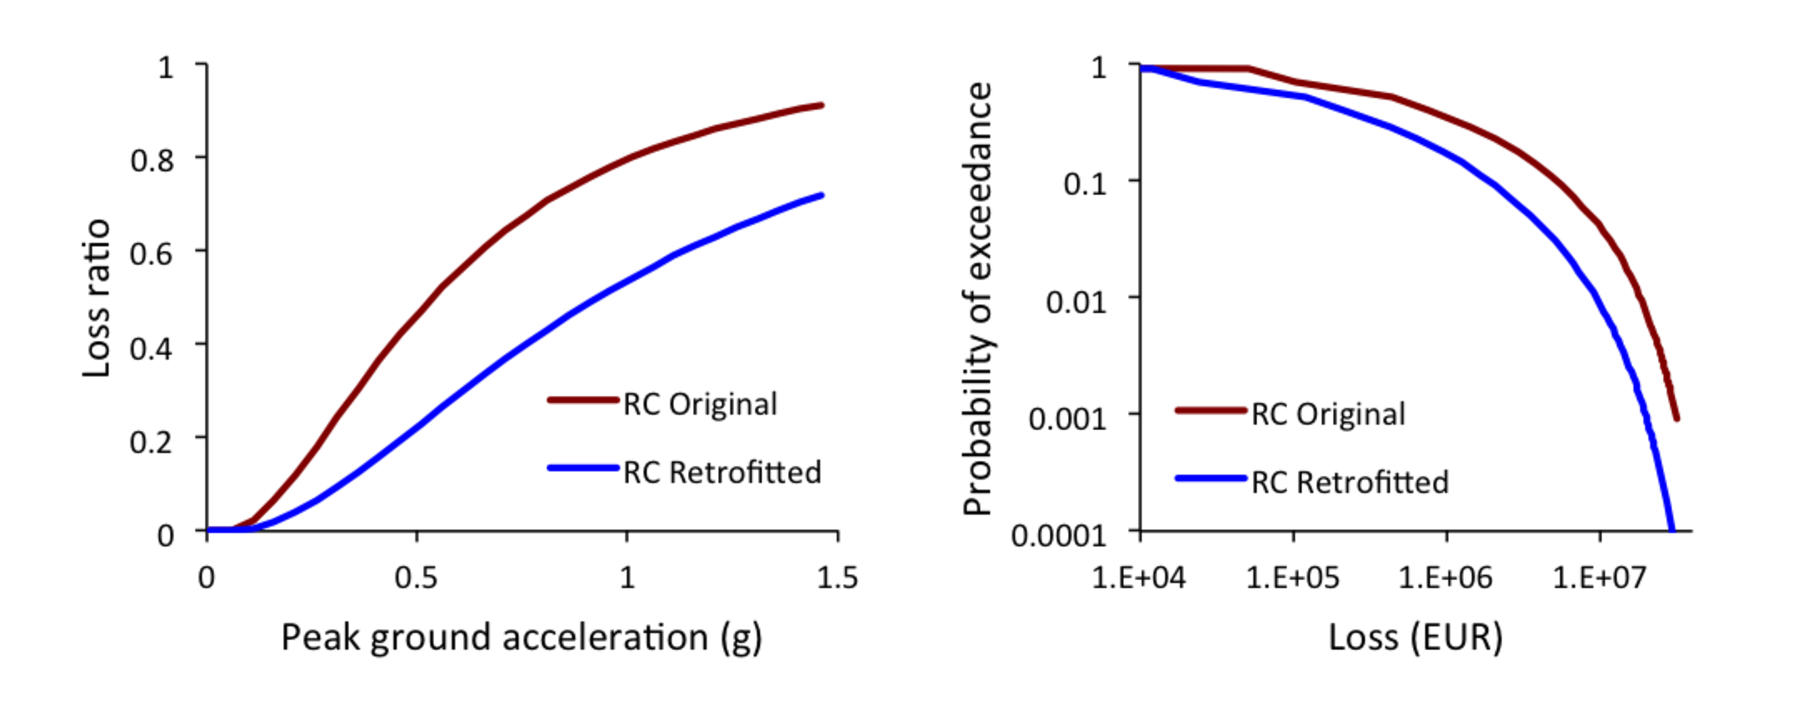
\includegraphics[width=12cm,height=5cm]{./figures/risk/VulnerabilityLosscurve.eps}
\caption{Vulnerability functions for the original and retrofitted configuration of a class of RC buildings (left) and respective loss exceedance curves (right).}
\label{fig:VulLosscurve}
\end{figure}

\item Then, an average annual loss ($AAL$) for each vulnerability configuration is calculated by numerically integrating the respective loss exceedance curve.  

\item For the calculation of the economic benefit $B$, the following formula can be employed:

\begin{equation}
B=(AAL_{retrofitted}-AAL_{original})\times\frac{1-e^{rt}}{r}
\end{equation}

where $r$ represents the inflation rate, which serves the purposes of considering the variation of the economic value of the \glspl{asset} during their life expectancy, or design life ($t$).

\item Finally, the previously defined benefit ($B$) is divided by the retrofitting cost ($C$), leading to the benefit/cost ratio ($BCR$). This process is repeated for all the \glspl{asset} comprised in the \gls{exposure model}.

\end{enumerate}

\section{Calculator Output}
The results of this calculator are stored in a benefit/cost ratio map, which includes the $AAL_{retrofitted}$, $AAL_{original}$ and the resulting $BCR$ at each location. In Figure \ref{fig:BCRMap}, a map of benefit/cost ratios for RC residential buildings in Nepal is presented.

\begin{figure}[ht]
\centering
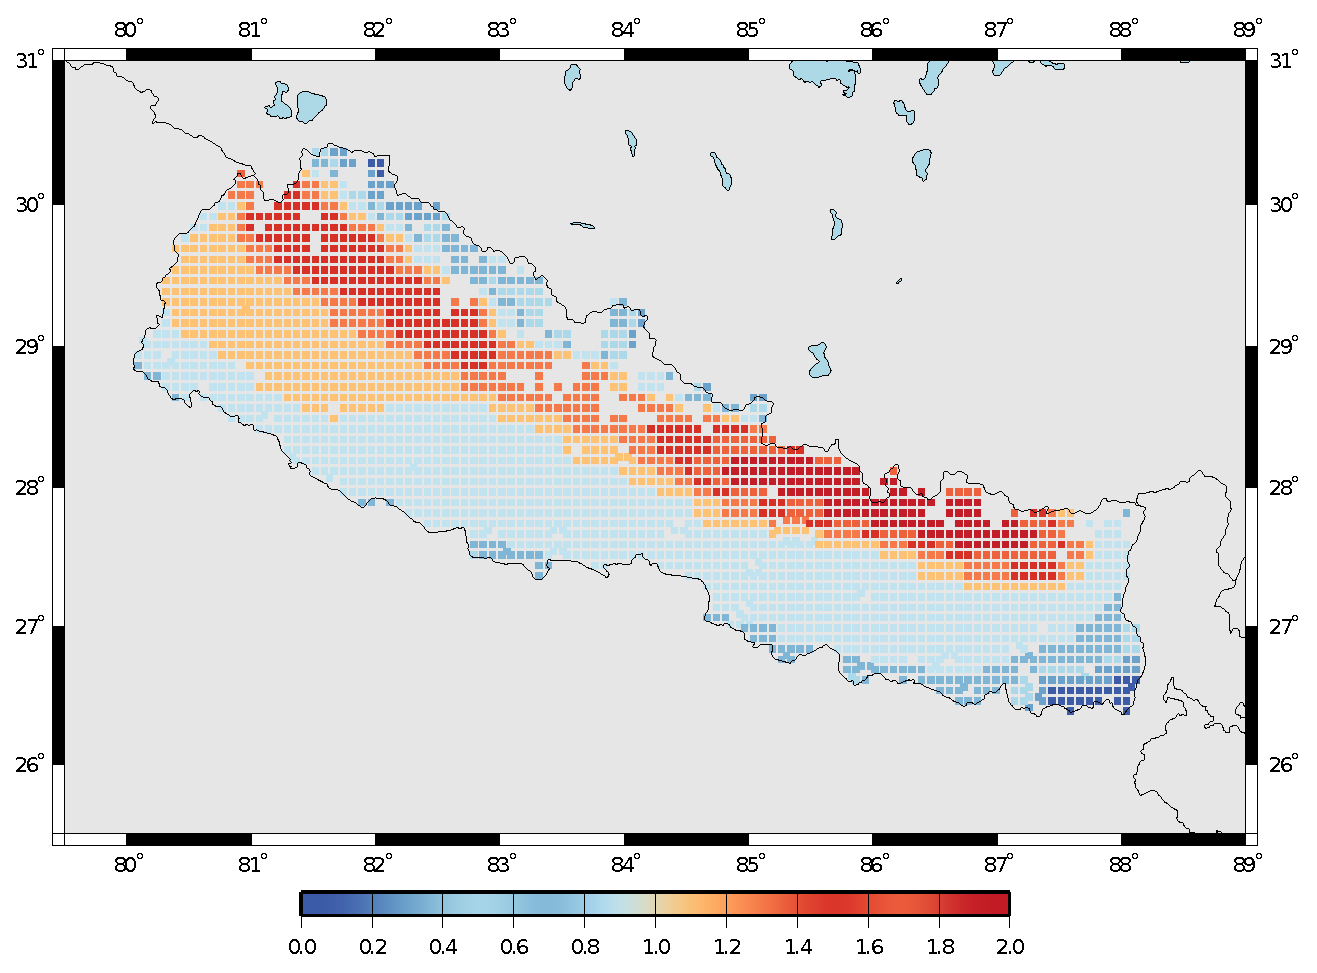
\includegraphics[width=12cm,height=8cm]{./figures/risk/BenefitCostRatioMap.eps}
\caption{Retrofitting benefit/cost ratio map for residential buildings in Nepal.}
\label{fig:BCRMap}
\end{figure}
% ==============================================================================
% ------------------------------------------------------------------------- Part
%\part{Socio-Economic Impact Assessment}
%	\glsdesc{acr:oqe} is the seismic hazard and risk calculation software developed by
the \glsdesc{acr:gem}. By following current standards in software
developments like test-driven development and continuous integration, the
\glsdesc{acr:oqe} aims at becoming an open, and community-driven tool for
seismic hazard and risk analysis.

The source code of the \glsdesc{acr:oqe} is available on a public web-based
repository at the following address:

\href{http://github.com/gem/oq-engine}{http://github.com/gem/oq-engine}.


% ------------------------------------------------------------------------------
\section{Running the OpenQuake-engine}
\index{Running OpenQuake!introduction}
\label{sec:running_oq_engine}

An \gls{acr:oqe} analysis is launched from the command line of a terminal.

A schematic list of the options that can be used for the execution of the
\gls{acr:oqe} can be obtained with the following command:

\begin{minted}[fontsize=\footnotesize,frame=single,bgcolor=lightgray]{shell-session}
user@ubuntu:~\$ oq-engine --help
\end{minted}

The result is the following:

\inputminted[firstline=1,fontsize=\footnotesize,frame=single]{shell-session}{oqum/help.txt}\\

% ------------------------------------------------------------------------------
\section{Concurrent Computing with OpenQuake}
\label{sec:concurrent_tasks}

The \glsdesc{acr:oqe} supports concurrent computing on both standalone
computers and computer clusters.

The \glsdesc{acr:oqe} works by splitting a computation into a number of tasks
which are then processed in parallel. The user has the ability to control the
splitting procedure, at least to a certain extent, by setting the parameter
`concurrent\_tasks` in the job.ini file. The \glsdesc{acr:oqe} will try to
produce a number of tasks close to `concurrent\_tasks`: it could be more, it
could be less. The details of the algorithm used can change depending on the
release of the engine and this is why they are not documented here. Instead,
we will document how you can set the parameter to a sensible value.

For instance, suppose you have a standard PC with an i7 processor with 8
hyperthreaded cores, i.e. 4 real cores. You could set:

concurrent\_tasks = 16

and then each hyperthreaded core would process around 2 tasks, which is a
reasonable value. If your computation consumes a lot of memory, you could
increase `concurrent\_tasks`, thus producing more tasks of smaller size,
requiring less memory.

If you don't set the parameter, a default value is used. Currently the default
is set to 8 times the number of cores in your controller machine. This default
value for `concurrent\_tasks` is likely to change in the future and you should
not rely on it if you are using a computer cluster. If you are not using a
cluster, the default value should be a reasonable choice.

Now, suppose you have have a cluster with a controller node and 10 workers,
each of which has 8 hyperthreaded cores, making for 80 cores in total. In this
scenario you could set:

concurrent\_tasks = 160

If you did not set the parameter, the default (assuming 8 cores on the
controller machine) would be 8 * 8 = 64 tasks, which is not enough. The number
of available cores on the workers is 80, so 16 cores will remain unused. Our
suggestion is to provide a value:

concurrent\_tasks = 2 * number of (hyperthread) cores in the workers

or more, if the computation has memory issues. With more tasks, less memory is
used, but more data is transferred and the computation becomes slower.

If `concurrent\_tasks` is set to zero, the parallelization is disabled and the
job is executed by using a single core. This is useful when debugging errors.

% ==============================================================================
% ------------------------------------------------------------------------- Part
%\part{Modeller's Toolkit}
% ------------------------------------------------------------------------------
%\chapter{Introduction}
%	\glsdesc{acr:oqe} is the seismic hazard and risk calculation software developed by
the \glsdesc{acr:gem}. By following current standards in software
developments like test-driven development and continuous integration, the
\glsdesc{acr:oqe} aims at becoming an open, and community-driven tool for
seismic hazard and risk analysis.

The source code of the \glsdesc{acr:oqe} is available on a public web-based
repository at the following address:

\href{http://github.com/gem/oq-engine}{http://github.com/gem/oq-engine}.


% ------------------------------------------------------------------------------
\section{Running the OpenQuake-engine}
\index{Running OpenQuake!introduction}
\label{sec:running_oq_engine}

An \gls{acr:oqe} analysis is launched from the command line of a terminal.

A schematic list of the options that can be used for the execution of the
\gls{acr:oqe} can be obtained with the following command:

\begin{minted}[fontsize=\footnotesize,frame=single,bgcolor=lightgray]{shell-session}
user@ubuntu:~\$ oq-engine --help
\end{minted}

The result is the following:

\inputminted[firstline=1,fontsize=\footnotesize,frame=single]{shell-session}{oqum/help.txt}\\

% ------------------------------------------------------------------------------
\section{Concurrent Computing with OpenQuake}
\label{sec:concurrent_tasks}

The \glsdesc{acr:oqe} supports concurrent computing on both standalone
computers and computer clusters.

The \glsdesc{acr:oqe} works by splitting a computation into a number of tasks
which are then processed in parallel. The user has the ability to control the
splitting procedure, at least to a certain extent, by setting the parameter
`concurrent\_tasks` in the job.ini file. The \glsdesc{acr:oqe} will try to
produce a number of tasks close to `concurrent\_tasks`: it could be more, it
could be less. The details of the algorithm used can change depending on the
release of the engine and this is why they are not documented here. Instead,
we will document how you can set the parameter to a sensible value.

For instance, suppose you have a standard PC with an i7 processor with 8
hyperthreaded cores, i.e. 4 real cores. You could set:

concurrent\_tasks = 16

and then each hyperthreaded core would process around 2 tasks, which is a
reasonable value. If your computation consumes a lot of memory, you could
increase `concurrent\_tasks`, thus producing more tasks of smaller size,
requiring less memory.

If you don't set the parameter, a default value is used. Currently the default
is set to 8 times the number of cores in your controller machine. This default
value for `concurrent\_tasks` is likely to change in the future and you should
not rely on it if you are using a computer cluster. If you are not using a
cluster, the default value should be a reasonable choice.

Now, suppose you have have a cluster with a controller node and 10 workers,
each of which has 8 hyperthreaded cores, making for 80 cores in total. In this
scenario you could set:

concurrent\_tasks = 160

If you did not set the parameter, the default (assuming 8 cores on the
controller machine) would be 8 * 8 = 64 tasks, which is not enough. The number
of available cores on the workers is 80, so 16 cores will remain unused. Our
suggestion is to provide a value:

concurrent\_tasks = 2 * number of (hyperthread) cores in the workers

or more, if the computation has memory issues. With more tasks, less memory is
used, but more data is transferred and the computation becomes slower.

If `concurrent\_tasks` is set to zero, the parallelization is disabled and the
job is executed by using a single core. This is useful when debugging errors.

% ------------------------------------------------------------------------------
%\chapter{Input visualization and preparation}
%	\input{./oqb/part_Modellers_Toolkit/input.tex}
% ==============================================================================
% ------------------------------------------------------------------------------
% ------------------------------------------------------------------------- Part
%\part{Appendixes}
%\appendix
% ------------------------------------------------------------------------------
%\chapter{nrML}
%	\input{./oqb/part_Appendix/nrML.tex}
% ------------------------------------------------------------------------------
%\chapter{Example of OpenQuake risk calculation configuration file}
%	\input{./oqb/part_Appendix/appendixHazardInputExample.tex}
% ==============================================================================
% ----------------------------------------------------------------- Bibliography
\small
\bibliographystyle{apalike}
\bibliography{./Bibliography/hazard,./Bibliography/risk,./Bibliography/sei.bib}
\normalsize
% ==============================================================================
% ------------------------------------------------------------------------ Index
\printglossaries
\printindex
\cleardoublepage
% Final empty page
\hfill \\ \thispagestyle{empty} \clearpage 
% ==============================================================================
% ------------------------------------------------------------------- Back Cover
\newgeometry{hmargin={0cm,-0.4cm},height=29.7cm}
\thispagestyle{empty}
\psset{unit=1cm}
\begin{pspicture}(0,0)(21cm,29.7cm)
	\psframe[fillstyle=solid,linecolor=cyan,fillcolor=white]
		(0.0cm,0.0cm)(21cm,15.0cm)
	\psframe[fillstyle=solid,linecolor=white,fillcolor=white]
		(0.0cm,15.0cm)(21cm,29.7cm)
	\psframe[fillstyle=solid,linecolor=blue01,fillcolor= blue01]
		(0.0cm,15.0cm)(21cm,15.5cm)
	\psframe[fillstyle=solid,linecolor=blue01,fillcolor= blue01]
		(0.0cm,25.0cm)(21cm,25.1cm)
\end{pspicture}
%
\end{document}
